\normaltrue \difficilefalse \tdifficilefalse
\correctionfalse

%\UPSTIidClasse{11} % 11 sup, 12 spé
%\newcommand{\UPSTIidClasse}{11}

\exer{Représentation 2D$\star$ \label{E2:05:1013}}
\setcounter{question}{0}\UPSTIcompetence[2]{E2-05}
\index{Compétence E3-05}
\index{Représentation 2D}

\ifcorrection
\else
\marginnote{\textbf{Pas de corrigé pour cet exercice.}}
\fi


\ifprof 
\else
Soit la pièce suivante.
\begin{center}
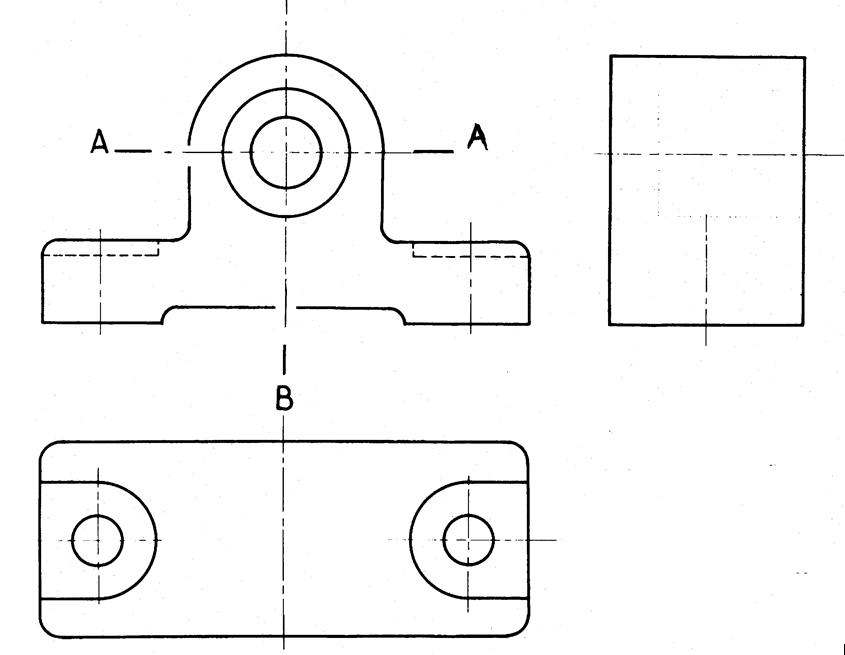
\includegraphics[width=\linewidth]{01}
\end{center}
 \fi
 
\question{Compléter les vues précédentes.}
\ifprof\begin{center}
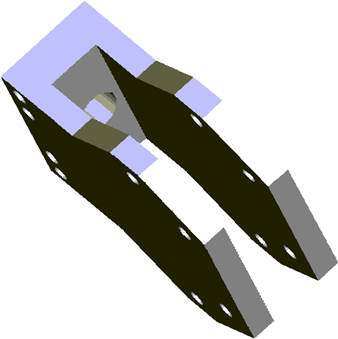
\includegraphics[width=.9\linewidth]{01_cor}
\end{center}
\else 
\fi

\ifprof
\else
\begin{flushright}
\footnotesize{Corrigé  voir \ref{E2:05:1013}.}
\end{flushright}%
\fi